\documentclass[conference]{IEEEtran}


\newcommand{\todo}[1]{\textcolor{cyan}{\textbf{[#1]}}}
\newcommand{\jayme}[1]{\textcolor{red}{{\it [Jayme says: #1]}}}
\newcommand{\scott}[1]{\textcolor{green}{{\it [Scott says: #1]}}}
\newcommand{\dan}[1]{\textcolor{blue}{{\it [Dan says: #1]}}}
\newcommand{\sam}[1]{\textcolor{green}{{\it [Sam says: #1]}}}


%\usepackage{hyperref}
\usepackage{url}
\usepackage{times}
\usepackage{balance}
\usepackage{color}
\usepackage{pgfplots}
\usepackage[justification=centering]{caption}

\usepackage{soul,color} % Used for highlighting text

% \hypersetup{bookmarks={false}}

\begin{document}
%

\title{Enhancing the Educational Experience for Deaf and Hard of Hearing Students in Software Engineering}

\author{\IEEEauthorblockN{Daniel E. Krutz, Samuel A. Malachowsky, and Scott D. Jones}
\IEEEauthorblockA{Software Engineering Department\\
Rochester Institute of Technology, USA\\
\{dxkvse, samvse, sdj2964\}@rit.edu}
\and
\and
\IEEEauthorblockN{Jayme A. Kaplan}
\IEEEauthorblockA{St. Mary's School for the Deaf\\
Buffalo, NY, USA\\
Jayme.Kaplan@gmail.com\\
}}

\maketitle


\begin{abstract}
Software engineering is largely a communication-driven, team-oriented discipline. There are numerous hurdles for ensuring proper communication and interaction between all project stakeholders, including physical, technological, and cultural barriers. These obstructions not only affect software engineering in industry, but in academia as well. One possible issue that is often overlooked in software engineering education is how to best educate Deaf and hard-of-hearing (Deaf/HoH) students, and how to fully engage them in the classroom.

In this paper, we present our experiences in teaching software engineering to Deaf/HoH students. In the classroom, these students work very closely in activities and on project teams with their hearing peers. We also present recommendations for creating a more robust software engineering educational experience for not only Deaf/HoH students, but for hearing students as well.

We encourage instructors not only in software engineering programs, but in other computing disciplines to consider our recommendations and observations in order to enhance the educational experience for all students in the classroom, whether Deaf/HoH or hearing.

\end{abstract}



\section{Introduction}

Efficient and effective communication is an integral part of most software projects. This includes proper communication between all stakeholders of the project --- customers, management, users, and developers. Communication is also very important in the educational process, between instructors and students, and between student peers. This is often made more difficult with the different communication abilities of students and instructors.

%The National Postsecondary Student Aid Study reported that 136,000 postsecondary students were Deaf/HoH in the 2007-2008 academic year with this number only expected to grow~\cite{nicab2008}.\dan{Probably a good idea to update this}

A recent study by Gallaudet University reported that between 9 and 22 people out of every 1,000 in the United States have a severe hearing impairment~\cite{deaf_stats_url}. Even with the availability and effectiveness of sign language interpreters to assist student and faculty communication, the educational experience is typically significantly hindered for both Deaf/HOH students and their hearing classmates. Studies have found that Deaf/HoH students were only comprehending 50-80\% of interpreted or assisted lectures, in comparison to 84-95\% from their hearing peers~\cite{Marschark_bibtex, Marschark02102008}. Universities across the United States face considerable challenges in educating students with disabilities in computing fields~\cite{Cavender:2009:SAA:1508865.1509043}. Students with disabilities are much less likely to pursue careers in computer science and engineering, and the dropout rate for these students is high~\cite{4418169, national2000women, Bueno:2007:ALA:1268784.1268903}.

The Software Engineering Department at the Rochester Institute of Technology (RIT) is the first and largest undergraduate program of its kind in the United States~\cite{lutz2012instilling}. RIT is also home to the National Technical Institute for the Deaf (NTID), with a goal of providing technical and professional education to Deaf/HoH students, with over 1,500 Deaf/HoH student enrollees~\cite{ntidurl}. Even though NTID is a separate college from the rest of the university, its students often attend classes with hearing students. Interpreters and other necessary resources are made available to all students on an on-demand basis. They are available for classroom lectures and activities, team project time outside of class, or whenever else they are requested by the student. NTID is a two-year college, so many of its students will transition to one of the many other colleges at RIT (including Software Engineering). Additionally, not all Deaf/HoH students at RIT begin their college career in NTID.

Software engineering is a team and communication-driven discipline~\cite{Pieterse:2006:SET:1216262.1216282}. At the Software Engineering department at RIT, our courses typically include a team project component. These teams may be comprised of both hearing and Deaf/HoH students. Other than the additional resources such as interpreters provided by the university, Deaf/HoH students are treated just like any other students in the program. While we have achieved a considerable amount of success educating students with hearing loss in our software engineering program, we have also faced significant hurdles. Despite the best efforts of the interpreters, Deaf/HoH students are prone to losing a large amount of both verbal and nonverbal communication through an interpreter. Group discussions and multiple conversations are largely impossibly for interpreters to fully communicate to the Deaf/HoH students~\cite{johnhopkins_data_URL}.

This work is not only aimed at helping Deaf/HoH students and faculty, but their hearing counterparts as well. In both academia and in industry, students are very likely to work with differently abled coworkers, bosses, and customers, which may include visual or other physical impairments, including hearing. Students need to learn to effectively and efficiently work with a diverse set of people. Not doing so will not only limit their effectiveness in the workplace, but also limit the people they are able to work with.

In the following paper, we discuss some of our experiences and future work in creating the most robust educational experience as possible for our Deaf/HoH students in the software engineering educational process along with observations and recommendations from a Speech Language Pathologist (SLP). We propose the following work in the hope that it may assist instructors and students at other institutions.  The specific goals of this work are to:

\begin{itemize}
\itemsep.5em
  \item Share our experiences in instructing Deaf/HoH students in the field of software engineering.
  \item Create a~\emph{Best Practices} guide for instructors.
  \item Discuss common mistakes in educating Deaf/HoH students.
  \item Discuss improvements to be made, both at our institution and others.
  \item Lay the groundwork for future work in this area.
\end{itemize}

The remainder of this paper is organized as follows: Section~\ref{sec: ourexperiences} describes our experiences and lessons learning with instructing Deaf/HoH students. Section~\ref{sec: recs} provides recommendations for students and instructors when interacting with Deaf/HoH students. Section~\ref{sec: relatedwork} provides a list of related works. Section~\ref{sec: futurework} addresses limitations and future research to be conducted, and Section~\ref{sec: conclusion} summarizes the findings of this work.

% Teams are important in software engineering education
% \cite{5319505}
% \cite{1158712}
% How do teams typically communicate in SE
% How to improve deaf education
% \cite{6297673}


\section{Our Experiences}
\label{sec: ourexperiences}

In order to understand the perspectives of faculty and hearing and Deaf/HoH students, we asked each group to fill out an anonymous survey based upon their experiences. For both the hearing and Deaf/HoH student participants, we sought a wide and diverse range of students.  The students ranged from freshmen to seniors, and some had profound hearing loss while others were able to hear through the use of hearing aids or cochlear implants~\cite{Zdenek:2007:FEV:1297144.1297198}.

%Some students that wear hearing aids or cochlear implants are more likely to mesh well with the other members of their group and with their respective faculty members. This is because these Deaf people are more confident advocating for themselves and are better able to communicate with their peers. Again, this is largely a case-by-case basis. Other factors included the respective student's confidence in themselves. In a learning environment many of the Deaf students do not speak up for themselves for fear of asking "a stupid question" and subsequently lose faith in their own education. This is the job of the educator and the faculty to prevent this from happening. Hearing students that were polled said that when Deaf students advocated for themselves and made it more clear of their needs, the group work proceeded much more smoothly.
%\dan{Is this the most appropriate place for this?}

In the following section, we will discuss some of the student and instructor feedback we received.

\subsection{Student Deaf/HoH Feedback}

We first asked Deaf/HoH about some of their biggest communication challenges in their courses. Some responses were:

\begin{quotation}
``It's hard for all of us as a whole including hearing [people]. We may have an increase in difficulty in communicating with our professors because some of them speak at the speed of light, while others have heavy accents.''
\end{quotation}

\begin{quotation}
``The biggest challenge I had during class was trying to figure out the instructions given to me from the professor.''
\end{quotation}

% Non Hearing
% Had trouble getting interpreters for their meetings
% Could only understand one portion the conversation at a time. Lost much information in team meetings.
%x Most students felt unwelcomed on the team. Team members didn't want to be assigned with them.
% Interpreter requests are time consuming.
% Teammates didn't know how to deal with them.
% Get to know hearing students to remove ignorances. Become friends with them. Show them that you are not "weird"
% Deaf students need to speak up
% Want to participate just like anyone else, but sometimes find it impossible or their teammates unwilling.
% Students want to perticpilate very much, and have more input, but are unable to do so.


The Deaf/HoH students provided very mixed reviews regarding their software engineering experiences. While several students provided very positive experiences, others expressed concerns and displeasure over their experiences. Very early in the team-based project component of many courses, many Deaf/HoH students felt unwelcome by their hearing teammates. They immediately felt like others in their team largely viewed them and their disability as a burden and many hearing students wished to avoid being on teams with them. Deaf/HoH students felt that their teammates did not know how to deal with them, and were largely ignorant of how to communicate, interact, or even act around them.

While even a small level of ignorance is not desired, it is expected. What is the significant amount of reported ignorance at an institute such as RIT, where a significant portion of the student body is Deaf/HoH. This problem is likely much more profound at other institutes without so many Deaf/HoH people in the student body.

One of the recommendations that Deaf/HoH students had for helping to limit this ignorance by having the two groups of students perform team-building exercises, getting to know one another before the start of the group activity. One student stated:

\begin{quotation}
``Generally, we [Deaf/HoH students] just need exposure. Both sides need to be willing to communicate. And sometimes, a student just isn't a good student, which reflects badly on one side. Feeling a connection (for example, becoming friends) is really helpful. Get to know the other person. Do team-building exercises.''
\end{quotation}

Deaf/HoH students also stated that they have had good experiences when they've advocated for themselves, and been proactive in the work being done with their team. Some of the student quotes include:

\begin{quotation}
``I would recommend that they advocate for themselves as much as possible so as to ensure that they are included as much as possible in the team's work.''
\end{quotation}

\begin{quotation}
``I would say participate and communicate a lot. Take a leadership role! This is actually no different than a non-deaf person, but when there's a mixture of hearing and deaf students, communication is even more important. A mixture multiplies communication problems, so it's super-important to communicate well. Taking a leadership role means not just sitting there and expecting others to do the work. This is very hard in a classroom environment, unfortunately, but it needs to be done.''
\end{quotation}

%\begin{quotation}
%``I sign Pidgin Signed English, so I frequently find myself repeating myself toward the interpreter which results in embarrassing myself or felt that whatever I wanted to contribute [to the group] was no longer significant. So I end up [preferring] to type out my conversations on my laptop instead.''
%\end{quotation}

Many students also said that they preferred to use the note-taking service, as it helped them very much with reviewing the course material after lecture or lab hours. (Note-taking is a service provided by NTID in which a hearing student takes detailed notes, combining slides and spoken content.)

\begin{quotation}
``Notetaking helped a large amount! It was very nice and convenient to be able to go back and look at the material on my own time.''
\end{quotation}

\begin{quotation}
``I use the notes from the note-taker to review for quizzes and tests. Since I started doing that, I feel like I'm more able to contribute to the class or group.''
\end{quotation}

%Notetaking is just one of the many services that are provided by RIT and they serve a great many people over the course of the academic year. This combined with the Department of Access Services's interpreting staff account for nearly 6,000 hours of academics that are covered.


While RIT has a large and excellent group of interpreters which is readily and freely available to students upon request, there were still some issues. Many students described difficulties with attaining an interpreter for team meetings since they had to request one in advance. This posed a problem for shorter, ad-hoc team meetings, or ones scheduled with little notice. Some students also described issues with the lack of technical background most of the interpreters had. They were often unable to understand computing acronyms and terminology, leading to a large amount of communication loss in translation. While this is an issue which can certainly be examined, we sympathize with the interpreters because it is not reasonable to expect them to be an expert in such a wide-range of difficult, technical areas. Many Deaf/HoH students also stated that they did not utilize interpreting services made available by the University since they did not feel like they needed this assistance. Much of this feedback is surprising, especially considering RIT has one of the largest, if not the largest, set of interpreters available at any institution in North America. This leads us to believe that similar problems not only exist at other institutions, but may be even more profound.

\begin{table}[h!]
\vspace{-0.05in}
\caption{Example Questions: Deaf/HoH Students}
\vspace{-0.1in}
\begin{center}
   \begin{tabular}{ p{22em} | p{10em} }

   Question  & Responses \\ \hline \hline
	How was your overall experience with the other members of group projects? & Poor: 13\%, Neutral: 34\%, Good: 53\% \\ \hline
	During class time, do you feel that you are "in the loop" regarding the coursework? & Yes: 80\%, Sometimes: 13\%, No: 7\% \\ \hline
	During class time, do you feel that you are at the same level as your peers? & Yes: 60\%, Sometimes: 13\%, No: 27\% \\ \hline
	When working in a group, do you feel confident communicating with hearing team members? & Always: 40\%, Sometimes: 53\%, Rarely: 7\% \\ \hline

    \end{tabular}
\end{center}

\label{table:deafQuestions}
\vspace{-0.1in}
\end{table}

Most Deaf/HoH students indicated that they wanted to interact more with their team, but were unable to do so. Their team would often relegate the Deaf/HoH students to non-leadership roles so they would not have to interact with the team as much. In other situations, the communication lost through the use of an interpreter hindered their ability to interact more in team meetings. One reasonably simple recommendation is to have only one person on the team speaking at a given time, which would allow the single interpreter to not be overwhelmed with the virtually unachievable task of trying to relate several conversations at once. One student stated:

\begin{quotation}
``Communication was the main issue for me because everyone was talking at once and I was completely lost.''
\end{quotation}

Communication in the classroom and in smaller groups is paramount to the success of all students, especially those who are Deaf/HoH. Good communication comes from focus. Many of the Deaf/HoH students said that the learning material was rushed and unclear, which led to issues understanding the material and subsequently diminished their credibility during smaller ad-hoc group meetings. Students reported that the instructors would typically speak and perform an in-class demo at the same time. When the Deaf/HoH students tried to follow along with the demo, they cannot see the interpreter and the monitor, whiteboard, or projection screen at the same time.

Another issue that many Dm   eaf/HoH students discussed was lag time: the time that it takes for the interpreter to hear what another student, group, or the professor is saying and interpret it into sign language for the Deaf/HoH student to see. Even though the interpreters do their best, there is usually around a 2-3 second delay between what is said and what is signed. Regardless of this, Deaf/HoH students still were able to understand the information that was signed to them. Many of the Deaf/HoH students said that they thought the interpreters did a great job overall:

\begin{quotation}
``Yes, an interpreter was there to interpret in the classroom and made the communication go smoothly.''
\end{quotation}

\subsection{Hearing Student Feedback}

Creating a cohesive learning environment is important for both hearing and Deaf/HoH students. We created an anonymous survey asking hearing students about their experiences with working on a team comprised of both hearing and deaf/hard of hearing students and asked them to rate their experience as~\emph{below average},~\emph{average}, or~\emph{above average}. Table~\ref{table:hearingQuestions} illustrates that an overwhelmingly large portion (75\%) of hearing students rated their experiences as being below average. Based on the feedback attached to the survey, a large portion of negative feelings are due to extra time required to complete tasks due to the communication barrier. Most hearing students felt that properly run team meetings and better overall communication practices could have alleviated most of the issues.

% Hearing students are often apprehensive about having a Deaf/HoH student be a part of their group.

%\begin{figure}[h!]
%    \begin{tikzpicture}
%        \begin{axis}[
%            symbolic x coords={Below Average, Average, Above Average},
%            xtick=data, bar width=50, xlabel=Rating, ylabel=\% Responses
%          ]
%            \addplot[ybar,fill=blue] coordinates {
%                (Below Average,   75)
%                (Average,  13)
%                (Above Average,   13)
%            };
%        \end{axis}
%    \end{tikzpicture}

%\caption{Hearing Student Team Experiences}
%\label{fig:hearingstudent}
%\end{figure}

\begin{table}[h!]
\vspace{-0.05in}
\caption{Example Questions: Hearing Students}
\vspace{-0.1in}
\begin{center}
   \begin{tabular}{ p{22em} | p{10em} }

   Question  & Responses \\ \hline \hline
How would you rate your experience with teams comprised of both hearing and Deaf/HoH students? & Below Average: 75\%, Average: 13\%, Above Average: 13\% \\ \hline
Have you found that the services offered, such as an interpreter or notetaker, has been adequate to address your team needs? & Yes: 33\%, Somewhat: 67\%, No: 0\% \\ \hline
Did you typically have an interpreter at your meetings? & Yes: 25\%, No: 75\% \\ \hline

    \end{tabular}
\end{center}

\label{table:hearingQuestions}
\vspace{-0.1in}
\end{table}

%\begin{figure}[h!]
%\def\angle{0}
%\def\radius{3}
%\def\cyclelist{{"orange","blue","red","green"}}
%\newcount\cyclecount \cyclecount=-1
%\newcount\ind \ind=-1
%\begin{tikzpicture}[nodes = {font=\small}]
%  \foreach \percent/\name in {
%      13/Average,
%      75/Below Average,
%      13/Above Average
%    } {
%      \ifx\percent\empty\else               % If \percent is empty, do nothing
%        \global\advance\cyclecount by 1     % Advance cyclecount
%        \global\advance\ind by 1            % Advance list index
%        \ifnum3<\cyclecount                 % If cyclecount is larger than list
%         \global\cyclecount=0              %   reset cyclecount and
%          \global\ind=0                     %   reset list index
%        \fi
%        \pgfmathparse{\cyclelist[\the\ind]} % Get color from cycle list
%        \edef\color{\pgfmathresult}         %   and store as \color
%        % Draw angle and set labels
%        \draw[fill={\color!50},draw={\color}] (0,0) -- (\angle:\radius)
%          arc (\angle:\angle+\percent*3.6:\radius) -- cycle;
%        \node at (\angle+0.5*\percent*3.6:0.7*\radius) {\percent\,\%};
%
%       \node[pin=\angle+0.0*\percent*3.6:\name]
%         at (\angle+0.5*\percent*3.6:\radius) {};
%        \pgfmathparse{\angle+\percent*3.6}  % Advance angle
%        \xdef\angle{\pgfmathresult}         %   and store in \angle
%      \fi
%    };
%\end{tikzpicture}
%\caption{Hearing Student Team Experiences}
%\label{fig:hearingstudent}
%\end{figure}

Many hearing students feel that the Deaf/HoH student does not advocate for themselves in the group and therefore the other members of the group are lost on how to interact with the them. One student said:

\begin{quotation}
``My teammates and I ended up picking up the work the hard-of-hearing teammate would have completed because we did not want to fall behind on the project.''
\end{quotation}

Many hearing students also expressed issues in bringing the Deaf/HoH students up to speed whenever they met in a group. Most of these meetings were ad-hoc and therefore had to rely on other means to communicate since interpreters were not always available. When interpreters were requested for these meetings, many of the hearing students felt that they did very well in conveying the information to the Deaf/HoH students. Additionally, many of them felt like they did not do enough to accommodate the Deaf/HoH student and welcome them in their group. It was also mentioned that the flow of communication was significantly easier to facilitate if one of the members in the group knew sign language.

%\begin{quotation}
%``I didn't enjoy the experience because it was hard to communicate (because the deaf person had a hard time with both sign language and English) Normally, I would have been fine with the experience because I know ASL fluently.''
%\end{quotation}

\begin{quotation}
``It's nice to have an interpreter, but it's not always possible. I am not an interpreting major but I have been forced to do some amateur interpreting out of necessity.''
\end{quotation}

When group members communicated electronically with Google Docs or another form, documentation for their projects went much more smoothly.

\begin{quotation}
``Documentation [went much better] because almost all conversations were recorded electronically.''
\end{quotation}

Due to the risk of miscommunication and the effort required to include the Deaf/HoH person, it was easier to simply exclude them from the project by assigning them a less strenuous workload.

\begin{quotation}
``This [text-based communication] made it very difficult to explain assignments and the work we needed done - the [Deaf/HoH] student ended up doing almost no work on the project.''
\end{quotation}

Hearing students had their own struggles with incorporating the Deaf/HoH student in their work and their group. Having interpreters was a great help, but unfortunately the option was not always available. While none of the survey respondents questioned the quality of the interpreters, many felt that the lack of interpreters hurt their interactions. In many cases, the Deaf/HoH student felt that they did not need one and could communicate well enough without them, and thus did not request an interpreter for either their in class work, or their project work outside of class. Several hearing students stated that the lack of an interpreter really hurt their team communication. Other hearing students echoed the thoughts of the Deaf/HoH students in that communication was made more difficult since the interpreters did not understand, and therefore were not able to effectively interpret, a wide range of technical terms. One student stated:

\begin{quotation}
``Even though they tried their best, interpreters were unable to understand (and therefore) communicate many of the technical terms and ideas. Interpreters were not present for many of the meetings due to a variety of reasons. Maybe the deaf student did not request them or were not available due to ad-hoc meetings.''
\end{quotation}

Some hearing students acknowledged problems with how they treated a Deaf/HoH teammate. From the beginning of a team-based project, many hearing students felt that they did not do enough to welcome or gain understanding with the Deaf/HoH student who was working on their team. Even though this meant more actual assigned work for the hearing teammates, many felt that it was easier to simply ignore the Deaf/HoH students in their group and not make them as much of a part of the team as their hearing counterparts. Even though they could see that many of the Deaf/HoH students were trying to become more involved with team activities, many hearing students stated that they did not have the patience to work with or understand Deaf/HoH students and would not properly involve them with their team.

\begin{quotation}
``The increased difficulty in communication made it difficult to explain and assign work --- almost to the point where it was easier to just assign to someone else and not include the deaf student.''
\end{quotation}

\begin{quotation}
``There is a language barrier which prevents smooth in-person communication between team members. Deaf tend to be left out of conversations and ad-hoc decision making. The technology for smooth communication and interpreters are available ad-hoc and require extra planning. Typing is inefficient.''
\end{quotation}

Many hearing students also felt that Deaf/HoH students have learned to work autonomously from the rest of their team. Software engineering is largely a team-based exercise, which relies upon strong team cohesion to deliver a high quality product on time and on budget. Software engineers working away from the rest of their team goes against much of how we actually want to teach the students to create software using the proper engineering mindset.

Regardless of whether Deaf/HoH members are part of the team itself, team-related issues that need to be addressed during the course of a project still arise, ranging from the technical to personal and interpersonal issues. Learning how to properly address these situations is an important part of the learning process. Far too often, however, students would fail to address various issues with their Deaf/HoH teammates largely due to the communication barriers. As an example, many did not wish to involve a 3rd-party interpreter in possibly confrontational issues.

Even with a significant amount of communication and cultural differences to overcome, hearing students generally had a very positive experience when working with Deaf/HoH students. Many took the time to understand Deaf culture and learn American Sign Language (ASL) to varying degrees. Most hearing students acknowledged that Deaf/HoH students thought just like everyone else and, just like hearing teammates, some were good teammates and worked hard, while others did not try to contribute much to the team. Many students enjoyed the experience of working with a more diverse set of teammates.

\begin{quotation}
``I enjoyed it because it brought in a new perspective for the team to work with.  As a result, we were able to deliver high end products that met a larger scope of users.''
\end{quotation}

\begin{quotation}
``....it [working on a team with Deaf/HoH students] was a good experience that opens your eyes to how different people can be.''
\end{quotation}

This diversity had other positive effects for the team as well. One student stated that the extra documentation and extra focus on communication had a positive effect on their final product:

\begin{quotation}
``What went well is that they[Deaf/HoH] are just as capable as anyone else, and the fact that we are going at a slower pace allows for an actual full thought process to occur instead of trying to blaze through half-thought-out options.''
\end{quotation}

\subsection{Faculty Feedback}

%Seven faculty members from the Software Engineering department ranging from very experienced (30+ years) to newly %appointed faculty responded to our survey. Most of the faculty felt that the services offered by the university were %adequate.

We surveyed 7 Software Engineering faculty members about their experiences with having Deaf/HoH students in their class projects. A wide range of instructors responded to our questionnaire --- from brand new faculty to 30-year tenured faculty. In general, most instructors did not notice many significant abnormalities or problems with Deaf/HoH students in comparison to ones who were hearing. One common observation was that documenting classroom materials was a significant help in keeping everyone up to date.

\begin{table}[h!]
\vspace{-0.05in}
\caption{Example Questions: Faculty}
\vspace{-0.1in}
\begin{center}
   \begin{tabular}{ p{22em} | p{10em} }

   Question  & Responses \\ \hline \hline
Do you feel like you were adequately prepared to have a deaf/hard of hearing student in your class? & Yes: 33\%, Somewhat: 50\%, No: 17\% \\ \hline
Do you feel like there were provided sufficient resources to address the needs of the student, both in and outside of the classroom? & Yes: 83\%, Sometimes: 17\%, No: 0\% \\ \hline
As an instructor, have you used any resources offered for the support of deaf/hard of hearing students? & Yes: 17\%, No: 83\% \\ \hline

    \end{tabular}
\end{center}

\label{table:facultyQuestions}
\vspace{-0.1in}
\end{table}

Most of the feedback regarding the interpreters was very positive, with some instructors feeling that they were doing an excellent job with terminology, while others saying there were understandable difficulties. A common theme was that it was important to get the Deaf/HoH students involved in team-based projects and help to motivate their participation in groups. One example statement:

\begin{quotation}
``Be sure to include the students in group activities, etc. Sometimes it can be hard to distinguish between barriers or issues caused by the disability and individual personality traits of the student.''
\end{quotation}

Many faculty said that having a Deaf/HoH student in their classroom really made them rethink their method of communicating their curriculum to the class. Many of them took the feedback they received from the Deaf students to heart and improved their own methods of teaching:

\begin{quotation}
``Have the same expectations of Deaf/HoH students as you would anyone else. If extra time is needed on tests, follow that procedure (or any other accommodations listed). CC [closed caption] any video used. Don't speak to the board while lecturing, your other students will appreciate that too.''
\end{quotation}

Additionally, many of the RIT/NTID interpreters faced struggles within their own field. Three interpreters that were interviewed claimed that many of the instructors here at RIT do not fully understand how to teach Deaf/HoH students. This may stem from lack of experience or training, but this is something they say the majority of interpreters have noticed. It was suggested that a workshop for instructors and faculty would help immensely. They were informed that RIT did, in fact, provide workshops, but that workshops were not mandatory.

One other issue that was brought up was that in New York state, there is no certificate requirement for interpreting education. RIT does have RID (Registry of Interpreters for the Deaf) certified interpreters, but not all interpreters have this certification. There are different levels of certification: community interpreting is the most basic; medical and educational interpreting require a much higher level of certification. Some suggested that RIT could pay for the newer interpreter's certification tracks, which would lead to an increase in the quality of interpreters overall. RIT currently does not pay for certification fees, and this led to a lack of motivation to take the certification exams. This, combined with the fact that certification is not a job requirement has made certification a lower priority to many interpriters. Recently at RIT, the Promotion Career Ladder Committee (PCLC) was established, chartered with helping interpreters to pursue higher levels in their career and driving participation in their career. An increase in number of certified interpreters could improve the clarity of technical information interpreted for the Deaf/HoH student.

%Finally, an interesting request shared by many of the instructors was a short~\emph{best practices} guide for how to most appropriately educate and interact with Deaf/HoH students in the classroom.

% Should we have this section?
\subsection{Analysis}

Most faculty felt that the resources available to them for communicating their material to Deaf/HoH students was adequate enough for the Deaf/HoH students to succeed in and pass the course. Interestingly, most Deaf/HoH students reported that they felt the teacher's materials were unclear and very vague, some feeling that the information itself was vague and therefore was interpreted as vague. This can amount to a large roadblock in the success of these students in the academic learning environment.

% Faculty felt that resources offered by the university were adequate, but most hearing students felt they were not.



\section{Recommendations}
\label{sec: recs}

With an eye on the primary challenges shared by each party, shown in Figure~\ref{fig:PrimaryChallenges}, this section includes recommendations for each person or interaction: Instructors, Deaf/HoH Interaction, Classroom Lectures, Group Work, Deaf/HoH Students, and for all students based on our research. Many of these recommendations were derived from our own observations, best practices from previous publications, and recommendations from a Speech Language Pathologist.

\begin{figure}
\vspace{-0.05in}
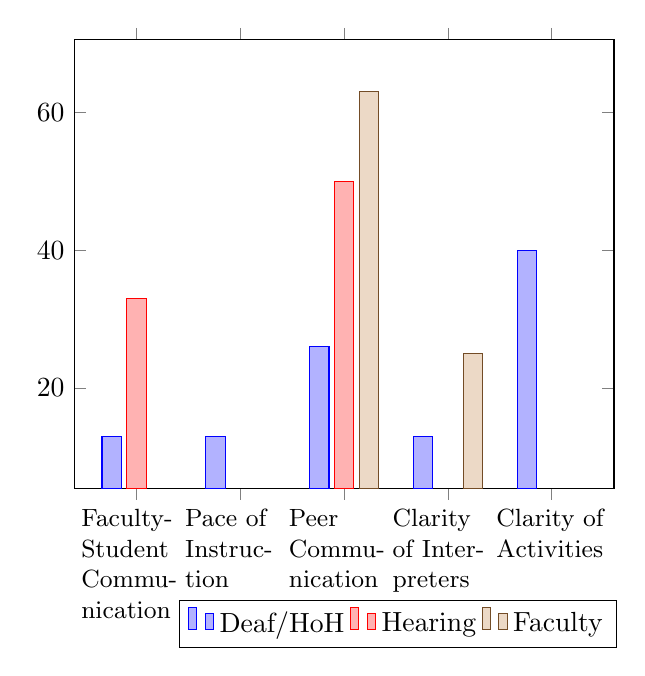
\begin{tikzpicture}
\begin{axis}[
    ybar,
%	scale only axis,
    enlargelimits=0.15,
    legend style={at={(0.6,-0.25)},
      anchor=north,legend columns=-1},
%   ylabel={\#participants},
    symbolic x coords={Faculty-Student Communication,Pace of Instruction,Peer Communication,Clarity of Interpreters,Clarity of Activities},
    xtick=data,
%    nodes near coords,
%    nodes near coords align={vertical},
	xticklabel style={text width=4em, font=\small}, 
	bar width=7pt
    ]
\addplot coordinates {(Faculty-Student Communication,13) (Pace of Instruction,13) (Peer Communication,26) (Clarity of Interpreters,13) (Clarity of Activities,40)};
\addplot coordinates {(Faculty-Student Communication,33) (Peer Communication,50)};
\addplot coordinates {(Clarity of Interpreters,25) (Peer Communication,63)};
\legend{Deaf/HoH,Hearing,Faculty}
\end{axis}
\end{tikzpicture}
\caption{Primary Challenges for Each Group (\%)}
\label{fig:PrimaryChallenges}
\end{figure}




%%%%

\subsection{For Instructors}

Working with a Deaf/HoH student is a new experience for many instructors. Teachers in the elementary and secondary levels have training on how to differentiate lessons and teach to a more diverse group of young people yet most still require support from specialized teachers or Teachers of the Deaf (TOD) to understand how to best educate Deaf/HoH students. At the university level, instructors are not typically versed in teaching philosophies and differentiation strategies, and do not have the strict support services from a TOD received by their elementary and secondary counterparts. Due to this, instructors entering a university where they may have students who are Deaf/HoH and are of mixed backgrounds, learning styles, and/or abilities may feel unprepared for differentiating their instruction style. They may also be unaware that small accommodations in the classroom can make for a much different communication and learning environment.

In this section we will discuss some measures instructors can take to communicate and teach more effectively to any class, but specifically classes of both hearing and Deaf/HoH students. A goal of this work is to assist instructors in the computing field in becoming more knowledgeable and understanding in ways they can help enhance the educational experience for students who are Deaf/HoH in their courses. Some general recommendations for interactions with Deaf/HoH individuals are:

%It is our hope that the field of computing continue to be inclusive and supportive to learners of different abilities.

\noindent
\textbf{General Interactions with Deaf/HoH individuals}
\begin{itemize}
\item When speaking with a Deaf/HoH individual, look at and speak to the individual not toward the interpreter. Speak clearly and naturally.
\item Keep sightlines open and clear from obstruction --- seeing the speaker's face is important for speechreading (lipreading) and nonverbal communication such as facial expressions.
\item Clarify/repeat messages and/or give examples. Allow for repetition of information, do not say ``never mind'' if the information was missed.
\item Deaf/HoH students may use different modes of communication: American Sign Language (ASL), Signed Exact English (SEE), Pidgin Signed English (PSE), Cued Speech, speechreading, and spoken/written English or other languages.

\item Deaf/HoH students may have access to auditory information via a hearing aid, cochlear implant and/or FM system. Each student will be different in their ability to utilize the auditory and spoken avenue for communication.
\item Familiarize yourself with Student Access \& Support Services and Disability Services available on campus (C-print, interpreting, note-taking, tutoring).
\item Students who are Deaf/HoH and also have an additional disability or blindness are know as ``Deaf Plus'' or ``Deafblind'' respectively. Numerous supporting resources may be found on on the web.
\footnote{\url{http://www.rit.edu/ntid/deafplus/about-website}}
\footnote{\url{http://www.ntid.rit.edu/support-services}}
\footnote{\url{http://www.rit.edu/studentaffairs/disabilityservices/info.php}}

 %Information on supporting ``Deaf Plus'' or ``Deafblind'' students in your classroom can be found in the Online Resources section below.
\end{itemize}

\noindent
\textbf{Classroom Lectures}\\
Dual or multi-directional attention is a huge barrier in a classroom for Deaf/HoH students. Dual attention refers to the consideration needed to attend to two stimuli simultaneously. Hearing people often do this with little effort (you may listen to a teacher while taking notes or looking at a handout). ``In contrast to hearing students who use dual channels --- auditory and visual --- for the input of classroom information, Deaf/HoH students tend to rely primarily on a single channel --- the visual channel.''~\cite{anissueoflearning_bibtex}. A classroom is full of auditory and visual channels that a Deaf/HoH learner must process through a mostly visual sense. ( i.e. watch an interpreter, see information on the board, take notes, and look at hand outs or a computer screen). For those with auditory access, they must also try to process the spoken message from the professor and filter out extraneous conversations and noises. All of this can be overwhelming when trying to focus on multiple channels simultaneously. This often results in the Deaf/HoH student missing information in one of these areas. The following are recommendations for ensuring quality classroom lectures:

\begin{itemize}
\item Talk with the Deaf/HoH student(s) about their communication preferences and needs.
\item Determine which services (if any) they will be using throughout the course (C-print, note-taking, interpreting, etc).
\item Allow them preferential seating.
\item Allow for all information to be accessed visually, (put everything up on the board, access slides on course website, etc.)
\item Face the class when speaking. Speak first, then write on the board, try not to speak while facing away from the class or writing information that the student will need to see at the same time.
\item Account for interpreter lag time. Although most skilled interpreters are extremely fast and efficient at relaying information, there will always be a bit of a lag time when interpreting. Time delay can affect turn taking and make it difficult to stay current in the conversation~\cite{Schick01012006}. Consider the situation where an instructor may call on a hearing student to answer a posed question before the interpreter has even finished signing the original question~\cite{IRRODL1015}.
\item Ask students to raise their hand and say who they are before speaking --- this is helpful for the student and/or interpreter to be able to indicate who is speaking and where the speaker is.
\item Provide notes and new vocabulary in advance. Pre-teach technical vocabulary if possible. Discuss vocabulary terms with interpreter (or student) prior to the lecture to ensure that the terms will be explained clearly.
\item Document the goings-on of the class and publish on a class website.
\item Design lesson plans in an organized, sequential manner.
\item Using a chat program or message board for discussions outside of class can help with communication process. Examples include Google Docs, Gchat, question forums, or online resources provided by your school.


\item If a student uses an amplification device:
\begin{itemize}
\item Cut down on extraneous noise (limit side conversations, limit shuffling of chairs, close doors/windows, etc.).
\item Consider students seating arrangements and allow for preferential seating.
\item Consider the acoustics of the classroom (tile flooring, humming computers, outdoor noises, sound reverberation, etc.)~\cite{soundproofing_bibtex}.
 \end{itemize}

\end{itemize}

\noindent
\textbf{Groups}\\
Group work can be one of the biggest challenges in a software engineering courses. Working in a mixed hearing and Deaf/HoH group makes communication more challenging. Faculty need to take the lead by setting up clear guidelines and make comments on interaction with clear reinforcement. One option is to create a point system for group involvement where bonus points are assigned based on collaborative accomplishments. If using this option, when group work is occurring in the classroom, wander around and assign extra points to those teams that are working collaboratively. Establish roles, responsibilities, and expectations in group interactions.   Encourage interaction amongst all group members.

Research shows that although giving communication strategies (turn taking, eye contact, facing toward communication partner, etc.) is important and useful for group work, it doesn't seem to be as powerful as using an overriding open/transparent way of communicating through technology. (i.e. g-chat, white board, Google Docs, question forums, etc.)~\cite{IRRODL1015}. The use of a chat program can help with communication by allowing each student the time to process the information and clearly communicate responses while working collaboratively. The level of complexity of communication goes up when everyone is involved and able to fully participate~\cite{IRRODL1015}.

Based upon some of the responses from our surveys, some recommendations are:
\begin{itemize}
\item Encourage Deaf/HoH students to take leadership roles within the group.
\item Get to know your group mates --- lead team-building exercises to encourage communication.
\item Maintain the same group for the semester --- once students set up working relationships with their group and develop communication strategies that work for them, encourage them to use the developed relationships to their advantage.
\item Deaf/HoH students should advocate for themselves as much as possible.

 \end{itemize}

\subsection{For Deaf or Hard of Hearing Students}

We next provide recommendations for Deaf/HoH students to ensure that they receive the best possible learning experience. To advocate for themselves, Deaf/HoH students may:

\begin{itemize}
\item Determine which access and support services will be most useful for you to utilize. Use them to support your work in lecture and group work.
\item Notify the professor of any and all services you are using and how they can support these services to the best of their abilities.
\item Inform the interpreter if you do not understand their signing, a term presented, or parts of the material.
\item Go to office hours, email, or communicate electronically with your instructors to discuss any questions or concerns you may have.
\item Explore other avenues of support for your communication needs within a group when an interpreter is unavailable to you. Consider researching which technological supports will work best for you, such as web-based chat programs or document programs (g-chat, Google Docs), text-to-voice/voice-to-text mobile or computer app options(C-Print, Dragon), and Video Remote Interpreting(VRI).
\item Develop communication rules or ``Communication Courtesy'' within a group. Examples could be:
	\begin{itemize}
	\item Acknowledging the speaker
	\item One person speaks at a time
	\item Raise hand to take a turn
	\item Limit interjections and distractions
	\item Utilize a note-taker in the group and share all notes
	\item Consider the environment, lines of sight, lighting, and acoustics
 \end{itemize}
 \end{itemize}

\subsection{For All Students}
It is important for all students in a group to feel that each group member is equally contributing. Each group member wants to feel valued and should be equally relied upon for work. Regardless of hearing status, if a member of a group is viewed as apart from the rest, excluded, not ``pulling their weight'', or not willing to collaborate or compromise, it will change the dynamics of the group and could result in a lower quality end product. All students need to learn how to work effectively in groups and develop strategies to ensure all group members fully participate and the work is completed to the standard of all group members. Learning how to properly address group situations and to work collaboratively is an integral part of the university learning experience.

\subsection{General Recommendations}
Based on the information collected from our surveys and research, we believe that further research and information is needed to determine the extent to which the following recommendations can be achieved:
\begin{itemize}
\item Instructors at universities with high concentrations of Deaf/HoH students should be required to take a workshop or course designed to introduce them to teaching Deaf/HoH students, give overview of support services available to students, and how to adjust the classroom environment to best support these students.
\item Technology-based departments should work more closely with the interpreters and the interpreting department to support terminology development for courses that contain jargon central to the subject.
\item Find better more user-friendly strategies for students in mixed hearing status groups, with the goal of allowing them to communicate freely and effectively.
 \end{itemize}

\section{Related Work}
\label{sec: relatedwork}

This paper represents the first known work on students with hearing loss and software engineering education. However, there are numerous previous papers that discuss Deaf/HoH education in computing. Ross~\cite{Ross:1982:TPD:964167.964174} described several methods of teaching programming to deaf students, one of which was through the use of a dynamic library of programming language examples. Other problematic areas for deaf students have also been conveyed, including difficulties with professional note-takers and interpreters due to their lack of a computer science background, resulting in a significant loss of information.

Cavender~\emph{et al.}\cite{Cavender:2009:SAA:1508865.1509043} described a 9-week summer program for students with hearing loss. This program is designed to provide a catalyst for the academic careers for Deaf/HoH students. This is largely accomplished through the use of tutors and mentors for these students, some of the lessons included the need to inform instructors on how to more properly educate Deaf/HoH students and the need to recruit tutors and mentors who are themselves differently abled so they may better relate to the students. One surprising finding is the communication variations which exist in the Deaf/HoH community along with the diversity of accommodation needs. Not all Deaf/HoH students possess the same sign language communication skills, nor do they necessarily have the same preference in sign languages. Students may communicate using American Sign Language (ASL), Signed Exact English (SEE), or ``Simultaneous Communication'' (Simcomm).

Burgstahler~\emph{et al.}~\cite{4418169} discussed several ways of increasing the participation of students with various disabilities in computing fields. Included in these was the collaboration and knowledge sharing of disability service programs across the United States where strategies for recruiting and retaining disabled students in computing fields is discussed. This work also stated that disabled students were underrepresented in computing and that increasing the participation of disabled students would require a collaborative effort from students, educators, and employers.

In order to assist educating Deaf/HoH students in computing disciplines, several papers have been written. Kheir and Way~\cite{Kheir:2007:IDS:1269900.1268860} discussed using real-time speech transcription in order to assist the inclusion of Deaf/HoH students in computer science courses. An affordable solution was described which greatly assisted HoH students in these computer science courses. Li and Xu~\cite{5454732} studied an inquiry-based teaching model for Deaf/HoH students. Inquiry-based teaching models are very student-oriented and allow students to investigate real-world computing problems under the direction of the course instructor. This research found that such a model would be beneficial for Deaf/HoH students.

Bueno~\emph{et al.}~\cite{Bueno:2007:ALA:1268784.1268903} described several methods of assisting instructors in adapting e-learning content. The primary contribution of this work was a tool which processes lecture text for Deaf/HoH students. This tool highlights words or expressions which are difficult to understand for Deaf/HoH students and links them to external visual resources. A visual resource is used because numerous studies have found that Deaf/HoH students who predominately communicate via sign language process images more efficiently than words~\cite{Santos}. This paper also discussed some of the manners in which Deaf/HoH students learned differently compared to hearing students. One example is the observation that Deaf/HoH students learn at their own pace which is very distinct from the pace of their hearing classmates~\cite{Bueno:2007:ECA:1268784.1268862}.

\section{Limitations \& Future Work}
\label{sec: futurework}

%While we have addressed many issues, there is still work to be done. Many of the Deaf/HoH population have their own preferred method of communication and some students prefer interpreters over one-on-one communication, but education for Deaf/HoH is a case-by-case basis (very much like their hearing peers) and there is no ``one size fits all'' approach. In this section, we discuss our plans for the future and how we hope this research will be applied not only to Software Engineering programs, but also other educational programs in different schools across the country.
%\todo{Add to the future work we will be doing}

While we have addressed a significant amount of issues for Deaf/HoH education, there is still a substantial amount of research to be done. While software engineering programs are rapidly growing from their beginnings in 1996~\cite{lutz2012instilling}, they still represent a minority of computing education fields worldwide. We believe, however, that a substantial portion of our lessons learned and recommendations will be applicable to not only other computing fields, but to a vast array of other programs as well. We surveyed a relatively large number of hearing and Deaf/HoH students and faculty, but this obviously represents only a very minor subset of these respective groups at only a single institution.

The use of technology and computing to support communication for Deaf/HoH individuals is an expanding field with innumerable other areas of research ranging from allowing hearing and Deaf/HoH to communicate using a Kinect~\cite{Chai:2013:VTS:2513383.2513398}, all the way to creating mobile devices which can assist Deaf/HoH individuals with medical responders~\cite{Buttussi:2010:UMD:1851600.1851605}. We understand that the use and development of new technologies and communication techniques will not replace the need for skilled interpreters who relay information clearly and effectively or improved methodologies and understanding by instructors and students. Deaf/HoH individuals are not members of a homogeneous group and each will have their own preferred method of communication. In the case of our students, some prefer to use interpreters over technologically-based communication, but education for all students is a case-by-case basis, regardless of hearing status, and there is no ``one size fits all'' approach.


% only SE
% only represent a small portion of the deaf community
% Still a substantical amount of research to be done



\section{Conclusion}
\label{sec: conclusion}
Deaf/HoH students are typically underrepresented and encounter significant hurdles in computing curriculums in higher education. In the Software Engineering department at RIT, we have a higher number of Deaf/HoH students than the typical university due to the presence of NTID on campus. While there are numerous challenges yet to be overcome, we hope that instructors and students will benefit from our work at other institutions. Additionally, we encourage further research and knowledge sharing in improvements to Deaf/HoH education, not only in software engineering, but in computing as a whole.


%\section*{Acknowledgement}
%Stuff
% Add a section about how this was supported by a grant from RIT
% I am intentionally leaving this out of the initial submission


\IEEEpeerreviewmaketitle


\balance
\bibliographystyle{abbrv}
\bibliography{SE_Deaf_Refs}




% that's all folks
\end{document}

% 2 = An Issue of Learning: The Effect of Visual Split Attention in Classes for Deaf and Hard of Hearing Students
% 8= http://www.acousticalsurfaces.com/soundproofing_tips/html/crashcourse.htm


%%%%%
% Make sure it is 8 pages?
%	Remove a refernce or two or make a foot note if I have to


%%%%%%
%	Add keywords?
%   Include some charts with data. 